\subsection{PUP}

\label{sec:pup}

The \index{PUP} PUP framework is a generic way to describe the data in an object and to use that description for any task requiring serialization.
The \charmpp\ system can use this description to pack the object 
into a message, and unpack the message into a new object on another 
processor. 
The name thus is a contraction of the words Pack and UnPack (PUP). 

Like many \CC\ concepts, the PUP framework is easier to use than 
describe: 

\begin{alltt}
class foo : public mySuperclass \{
 private:
    double a;
    int x;
    char y;
    unsigned long z;
    float arr[3];
 public:
    ...other methods...

    //pack/unpack routine: describe my fields to charm++
    void pup(PUP::er &p) \{
      mySuperclass::pup(p);
      p|a;
      p|x; p|y; p|z;
      PUParray(p,arr,3);
    \}
\};
\end{alltt}

This class's pup routine describes the fields of a \uw{foo} to \charmpp{}.
This allows \charmpp\ to: marshall parameters of type \uw{foo} across processors,
translate \uw{foo}s across processor architectures, read and write \uw{foo}s
to disk files, inspect and modify \uw{foo} objects in the debugger, and 
checkpoint and restart calculations involving \uw{foo}s.



\subsubsection{PUP contract}

Your object's pup routine must save and restore all your object's data.
As shown, you save and restore a class's contents by writing a routine c
alled ``pup'' which passes all the parts of the class to an object of type 
\index{PUP::er} \kw{PUP::er}, which does the saving or restoring.  
We often use ``pup'' as a verb, meaning ``to save/restore the value of''
or equivalently, ``to call the pup routine of''.

Pup routines for complicated objects normally call the pup routines
for their simpler parts.  Since all objects depend on their immediate
superclass, the first line of every pup routine is a call to the 
superclass's pup routine---the only time you shouldn't call your superclass's
pup routine is when you don't have a superclass.  If your superclass has
no pup routine, you must pup the values in the superclass yourself.


\paragraph{PUP operator}

\label{sec:pupstl}

The recommended way to pup any object \verb.a. is to use \verb.p|a;..
This syntax is an operator \verb.|. applied to the \kw{PUP::er} \verb.p.
and the user variable \verb.a..

The \verb.p|a;. syntax works wherever a is:

\begin{itemize}
 \item A simple type, including char, short, int, long, float, or double.
    In this case, \verb.p|a;. copies the data in-place.
    This is equivalent to passing the type directly to the \kw{PUP::er}   
       using \verb.p(a)..
 \item Any object with a pup routine.
    In this case, \verb.p|a;. calls the object's pup routine.
    This is equivalent to the statement \kw{a.pup(p);}. 
 \item A pointer to a PUP::able object, as described in Section~\ref{sec:pup::able}.
    In this case, \verb.p|a;. allocates and copies the appropriate subclass.
 \item An object with a \kw{PUPbytes}(\uw{myClass}) declaration in the header.
    In this case, \verb.p|a;. copies the object as plain bytes, like memcpy.
 \item An object with a custom \verb.operator |. defined.
    In this case, \verb.p|a;. calls the custom \verb.operator |..
\end{itemize}

For container types, you must simply pup each element of the container.
For arrays, you can use the utility routine \kw{PUParray}, which takes
the \kw{PUP::er}, the array base pointer, and the array length.
This utility routine is defined for user-defined types T as:
  \begin{alltt}
    template<class T>
    inline void PUParray(PUP::er &p,T *array,int length) \{
       for (int i=0;i<length;i++) p|array[i];
    \}
  \end{alltt}

If the variable is from the C++ Standard Template Library, you can include 
operator\verb.|.'s for STL vector, map, list, pair, and string, templated
on anything, by including the header ``pup\_stl.h''.

As usual in \CC{}, pointers and allocatable objects usually require special handling. 
Typically this only requires a \kw{p.isUnpacking()} conditional block, 
where you perform the appropriate allocation.  See 
Section~\ref{sec:pupdynalloc} for more information and examples.  

If the object does not have a pup routine, and you cannot add one or use 
PUPbytes, you can define an operator\verb.|. to pup the object.
For example, if \uw{myClass} contains two fields \uw{a} and \uw{b}, the 
operator\verb.|. might look like:

\begin{alltt}
  inline void operator|(PUP::er &p,myClass &c) \{
    p|c.a;
    p|c.b;
  \}
\end{alltt}


\paragraph{PUP as bytes}

\label{sec:pupbytes}

For classes and structs with many fields, it can be tedious and 
error-prone to list all the fields in the pup routine.
You can avoid this listing in two ways, as long as the
object can be safely copied as raw bytes---this is normally 
the case for simple structs and classes without pointers.

\begin{itemize}
\item Use the \verb.PUPbytes(myClass). macro in your header file.
      This lets you use the \verb.p|*myPtr;. syntax 
      to pup the entire class as sizeof(myClass) raw bytes.

\item Use \verb.p((void *)myPtr,sizeof(myClass));. in the pup 
      routine.  This is a direct call to pup a set of bytes. 
      
\item Use \verb.p((char *)myCharArray,arraySize);. in the pup 
      routine.  This is a direct call to pup a set of bytes. 
	  Other primitive types may also be used.
      
\end{itemize}

Note that pupping as bytes is just like using `memcpy': 
it does nothing to the data but copy it whole.
For example, if the class contains any pointers, you
must make sure to do any allocation needed, and
pup the referenced data yourself.

Pupping as bytes will prevent your pup routine from 
ever being able to work across different machine 
architectures.  We don't do this very often yet, but 
eventually may, so pupping as bytes is currently discouraged.



\paragraph{PUP overhead}

\label{sec:pupoverhead}

The \kw{PUP::er} overhead is very small---one virtual function call
for each item or array to be packed/unpacked.  The actual packing/unpacking is
normally a simple memory-to-memory binary copy. 

For arrays of builtin types like ``int" and ``double", or arrays of a type 
with the ``PUPbytes'' declaration, \kw{PUParray} uses an even faster block 
transfer, with one virtual function call per array.


\paragraph{PUP structured dagger}

\label{sec:pupsdag}

Please note that if your object contains Structured Dagger code (see section~\ref{sec:sdag}) you must call the generated routine \kw{\_\_sdag\_pup} to correctly pup the Structured Dagger state:

\begin{alltt}
class bar : public barParent \{
 public:
    bar_SDAG_CODE 
    ...other methods...

    virtual void pup(PUP::er& p) \{
      barParent::pup(p);
      __sdag_pup(p);
      ...pup other data here...
    \}
\};
\end{alltt}



\paragraph{PUP modes}

\label{sec:pupmodes}

\charmpp{} uses your pup routine to both pack and unpack, 
by passing different types of \kw{PUP::er}s to it.  The routine
\kw{p.isUnpacking()} returns true if your object is being unpacked---that 
is, your object's values are being restored.  Your pup routine must
work properly in sizing, packing, and unpacking modes; and
to save and restore properly, the same fields must be passed 
to the \kw{PUP::er}, in the exact same order, in all modes.
This means most pup routines can ignore the pup mode.

Three modes are used, with three separate types of \kw{PUP::er}: 
sizing, which only computes the size of your data without modifying it;
packing, which reads/saves values out of your data; and unpacking,
which writes/restores values into your data.  You can determine
exactly which type of \kw{PUP::er} was passed to you using the
\kw{p.isSizing()}, \kw{p.isPacking()}, and \kw{p.isUnpacking()}
routines. However, sizing and packing should almost always be 
handled identically, so most programs should use \kw{p.isUnpacking()}
and \kw{!p.isUnpacking()}.  Any program that calls \kw{p.isPacking()} 
and does not also call \kw{p.isSizing()} is probably buggy, because
sizing and packing must see exactly the same data.


The \kw{p.isDeleting()} flag indicates the object will be deleted
after calling the pup routine.  This is normally only needed for
pup routines called via the C or f90 interface, as provided by 
AMPI or the FEM framework.  Other \charmpp{} array elements, 
marshalled parameters, and other C++ interface objects 
have their destructor called when they are deleted, so the 
\kw{p.isDeleting()} call is not normally required---instead,
memory should be deallocated in the destructor as usual.


\subsubsection{Life Cycle}

\label{sec:lifecycle}

\begin{figure}[h]
\begin{center}
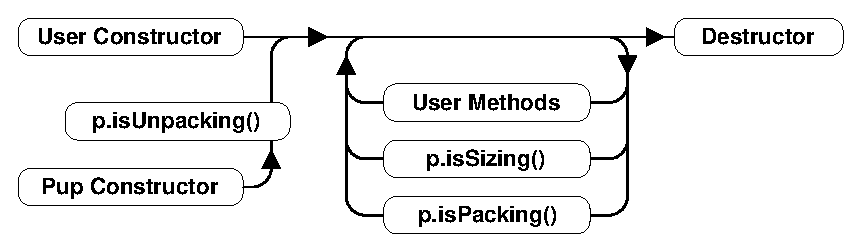
\includegraphics[width=6.0in]{fig/pup}
\end{center}
\caption{Life cycle of an object with a pup routine.}
\label{fig:pup}
\end{figure}

The life cycle of an object with a pup routine is shown in 
Figure~\ref{fig:pup}.  As usual in \CC{}, objects are 
constructed, do some processing, and are then destroyed.

Objects can be created in one of two ways: they can
be created using a normal constructor as usual; or they
can be created using their pup constructor.  The pup constructor
for \charmpp{} array elements and \kw{PUP::able} objects
is a ``migration constructor'' that takes a single ``CkMigrateMessage *";
for other objects, such as parameter marshalled objects,
the pup constructor has no parameters.  The pup constructor
is always followed by a call to the object's pup routine in
\verb.isUnpacking. mode.

Once objects are created, they respond to regular user methods
and remote entry methods as usual.  At any time, the object 
pup routine can be called in \verb.isSizing. or \verb.isPacking.
mode.  User methods and sizing or packing pup routines can be called
repeatedly over the object lifetime.

Finally, objects are destroyed by calling their destructor
as usual.



\subsubsection{Dynamic Allocation}

\label{sec:pupdynalloc}

If your class has fields that are dynamically allocated, when unpacking
these need to be allocated (in the usual way) before you pup them.
Deallocation should be left to the class destructor as usual.

\paragraph{No allocation}

The simplest case is when there is no dynamic allocation.
\begin{alltt}
class keepsFoo : public mySuperclass \{
private:
    foo f; /* simple foo object*/
public:
    keepsFoo(void) \{ \}
    void pup(PUP::er &p) \{
      mySuperclass::pup(p);
      p|f; // pup f's fields (calls f.pup(p);) 
    \}
    ~keepsFoo() \{ \}
\};
\end{alltt}

\paragraph{Allocation outside pup}

The next simplest case is when we contain a class 
that is always allocated during our constructor,
and deallocated during our destructor.  Then no allocation
is needed within the pup routine.
\begin{alltt}
class keepsHeapFoo : public mySuperclass \{
private:
    foo *f; /*Heap-allocated foo object*/
public:
    keepsHeapFoo(void) \{
      f=new foo;
    \}
    void pup(PUP::er &p) \{
      mySuperclass::pup(p);
      p|*f; // pup f's fields (calls f->pup(p))
    \}
    ~keepsHeapFoo() \{delete f;\}
\};
\end{alltt}

\paragraph{Allocation during pup}

If we need values obtained during the pup routine
before we can allocate the class, we must 
allocate the class inside the pup routine.
Be sure to protect the allocation with ``if (p.isUnpacking())''.
\begin{alltt}
class keepsOneFoo : public mySuperclass \{
private:
    foo *f; /*Heap-allocated foo object*/
public:
    keepsOneFoo(...) \{f=new foo(...);\}
    keepsOneFoo() \{f=NULL;\} /* pup constructor */
    void pup(PUP::er &p) \{
      mySuperclass::pup(p);
      ...
      if (p.isUnpacking()) /* must allocate foo now */
         f=new foo(...);
      p|*f;//pup f's fields
    \}
    ~keepsOneFoo() \{delete f;\}
\};
\end{alltt}

\paragraph{Allocatable array}

For example, if we keep an array of doubles,
we need to know how many doubles there are 
before we can allocate the array.  Hence we must
first pup the array length, do our allocation,
and then pup the array data.  We could allocate memory using 
malloc/free or other allocators in exactly the same way.
\begin{alltt}
class keepsDoubles : public mySuperclass \{
private:
    int n;
    double *arr;/*new'd array of n doubles*/
public:
    keepsDoubles(int n_) \{
      n=n_;
      arr=new double[n];
    \}
    keepsDoubles() \{ \} 
    
    void pup(PUP::er &p) \{
      mySuperclass::pup(p);
      p|n;//pup the array length n
      if (p.isUnpacking())  arr=new double[n];
      PUParray(p,arr,n); //pup data in the array
    \}
    
    ~keepsDoubles() \{delete[] arr;\}
\};
\end{alltt}

\paragraph{NULL object pointer}

If our allocated object may be NULL, our allocation
becomes much more complicated.  We must first check
and pup a flag to indicate whether the object exists, 
then depending on the flag, pup the object.
\begin{alltt}
class keepsNullFoo : public mySuperclass \{
private:
    foo *f; /*Heap-allocated foo object, or NULL*/
public:
    keepsNullFoo(...) \{ if (...) f=new foo(...);\}
    keepsNullFoo() \{f=NULL;\}
    void pup(PUP::er &p) \{
      mySuperclass::pup(p);
      int has_f=(f!=NULL);
      p|has_f;
      if (has_f) {
        if (p.isUnpacking()) f=new foo;
        p|*f;
      } else {
        f=NULL;
      }
    \}
    ~keepsNullFoo() \{delete f;\}
\};
\end{alltt}

This sort of code is normally much longer and more
error-prone if split into the various packing/unpacking cases.

\paragraph{Array of classes}

An array of actual classes can be treated exactly the same way
as an array of basic types.  PUParray will pup each 
element of the array properly, calling the appropriate \verb.operator|..
\begin{alltt}
class keepsFoos : public mySuperclass \{
private:
    int n;
    foo *arr;/*new'd array of n foos*/
public:
    keepsFoos(int n_) \{
      n=n_;
      arr=new foo[n];
    \}
    keepsFoos() \{ arr=NULL; \} 
    
    void pup(PUP::er &p) \{
      mySuperclass::pup(p);
      p|n;//pup the array length n
      if (p.isUnpacking())  arr=new foo[n];
      PUParray(p,arr,n); //pup each foo in the array
    \}
    
    ~keepsFoos() \{delete[] arr;\}
\};
\end{alltt}


\paragraph{Array of pointers to classes}

An array of pointers to classes must handle each element
separately, since the PUParray routine does not work with 
pointers.  An ``allocate'' routine to set up the array
could simplify this code.  More ambitious is to construct
a ``smart pointer'' class that includes a pup routine.
\begin{alltt}
class keepsFooPtrs : public mySuperclass \{
private:
    int n;
    foo **arr;/*new'd array of n pointer-to-foos*/
public:
    keepsFooPtrs(int n_) \{
      n=n_;
      arr=new foo*[n]; // allocate array
      for (int i=0;i<n;i++) arr[i]=new foo(...); // allocate i'th foo
    \}
    keepsFooPtrs() \{ arr=NULL; \} 
    
    void pup(PUP::er &p) \{
      mySuperclass::pup(p);
      p|n;//pup the array length n
      if (p.isUnpacking()) arr=new foo*[n]; // allocate array
      for (int i=0;i<n;i++) \{
        if (p.isUnpacking()) arr[i]=new foo(...); // allocate i'th foo
        p|*arr[i];  //pup the i'th foo
      \}
    \}
    
    ~keepsFooPtrs() \{
       for (int i=0;i<n;i++) delete arr[i];
       delete[] arr;
     \}
\};
\end{alltt}

Note that this will not properly handle the case where
some elements of the array are actually subclasses of foo,
with virtual methods.  The PUP::able framework described
in the next section can be helpful in this case.


\subsubsection{Subclass allocation via PUP::able}

\label{sec:pup::able}
If the class \uw{foo} above might have been a subclass, instead of
simply using \uw{new foo} above we would have had to allocate 
an object of the appropriate subclass.  Since determining the
proper subclass and calling the appropriate constructor yourself can be 
difficult, the PUP framework provides a scheme for automatically
determining and dynamically allocating subobjects of the appropriate type.

Your superclass must inherit from \kw{PUP::able}, which provides 
the basic machinery used to move the class.  
A concrete superclass and all its concrete subclasses require these
four features:

\begin{itemize}
\item A line declaring \kw{PUPable \uw{className};} in the .ci file.
This registers the class's constructor.

\item A call to the macro \kw{PUPable\_decl(\uw{className})} in the
class's declaration, in the header file.  This adds a virtual 
method to your class to allow \kw{PUP::able} to determine your class's type.

\item A migration constructor---a constructor that takes \kw{CkMigrateMessage *}.
This is used to create the new object on the receive side, immediately
before calling the new object's \kw{pup} routine.

\item A working, virtual \kw{pup} method.  You can omit this if your
class has no data that needs to be packed.
\end{itemize}

An abstract superclass---a superclass that will never actually be 
packed---only needs to inherit from \kw{PUP::able} and include a 
\kw{PUPable\_abstract(\uw{className})} macro in their body.  For
these abstract classes, the 
.ci file, \kw{PUPable\_decl} macro, and constructor are not needed.

For example, if \uw{parent} is a concrete superclass and \uw{child} its
subclass,

\begin{alltt}
//In the .ci file:
   PUPable parent;
   PUPable child; //Could also have said ``PUPable parent, child;''

//In the .h file:
class parent : public PUP::able \{
    ... data members ...
public:
    ... other methods ...
    parent() \{...\}
    
    //PUP::able support: decl, migration constructor, and pup
    PUPable\_decl(parent);  
    parent(CkMigrateMessage *m) : PUP::able(m) \{\}
    virtual void pup(PUP::er &p) \{
        PUP::able::pup(p);//Call base class
        ... pup data members as usual ...
    \}  
\};
class child : public parent \{
    ... more data members ...
public:    ... more methods, possibly virtual ...
    child() \{...\}
    
    //PUP::able support: decl, migration constructor, and pup
    PUPable\_decl(child);  
    child(CkMigrateMessage *m) : parent(m) \{\}
    virtual void pup(PUP::er &p) \{
        parent::pup(p);//Call base class
        ... pup child's data members as usual ...
    \}  
\};

\end{alltt}

With these declarations, then, we can automatically 
allocate and pup a pointer to a parent or child
using the vertical bar \kw{PUP::er} syntax, which on the receive
side will create a new object of the appropriate type:

\begin{alltt}
class keepsParent \{
    parent *obj; //May actually point to a child class (or be NULL)
public:
    ...
    ~keepsParent() \{
        delete obj;
    \}
    void pup(PUP::er &p) 
    \{
        p|obj;
    \}
\};
PUPmarshall(keepsParent);
\end{alltt}

This will properly pack, allocate, and unpack obj whether
it is actually a parent or child object.  The child class 
can use all the usual \CC\ features, such as virtual functions
and extra private data.

If obj is NULL when packed, it will be restored to NULL when unpacked.
For example, if the nodes of a binary tree are \kw{PUP::able},
one may write a recursive pup routine for the tree quite easily:

\begin{alltt}
// In the .ci file:
    PUPable treeNode;

// In the .h file
class treeNode : public PUP::able \{
    treeNode *left;//Left subtree
    treeNode *right;//Right subtree
    ... other fields ...
public:
    treeNode(treeNode *l=NULL, treeNode *r=NULL);
    ~treeNode() \{delete left; delete right;\}
    
    // The usual PUP::able support:
    PUPable\_decl(treeNode);
    treeNode(CkMigrateMessage *m) : PUP::able(m) \{ left=right=NULL; \}
    void pup(PUP::er &p) \{
        PUP::able::pup(p);//Call base class
        p|left;
        p|right;
        ... pup other fields as usual ...
    \}
\};
\end{alltt}

This same implementation will also work properly even if the tree's
internal nodes are actually subclasses of treeNode.

You may prefer to use the macros \kw{PUPable\_def(\uw{className})}
and \kw{PUPable\_reg(\uw{className})} rather than using \kw{PUPable}
in the .ci file.  \kw{PUPable\_def} provides routine definitions used
by the \kw{PUP::able} machinery, and should be included in exactly one
source file at file scope.  \kw{PUPable\_reg} registers this class
with the runtime system, and should be executed exactly once per node 
during program startup.

Finally, a \kw{PUP::able} superclass like \uw{parent} above 
must normally be passed around via a pointer or reference, because the object
might actually be some subclass like \uw{child}.  Because
pointers and references cannot be passed across processors,
for parameter marshalling you must use the special templated 
smart pointer classes \kw{CkPointer} and \kw{CkReference},
which only need to be listed in the .ci file.

A \kw{CkReference} is a read-only reference to a \kw{PUP::able} object---it
is only valid for the duration of the method call.  A \kw{CkPointer}
transfers ownership of the unmarshalled \kw{PUP::able} to the method, so the 
pointer can be kept and the object used indefinitely.  

For example, if the entry method \uw{bar} needs a \kw{PUP::able} \uw{parent}
object for in-call processing, you would use a \kw{CkReference} like this:

\begin{alltt}
// In the .ci file:
    entry void barRef(int x,CkReference<parent> p);

// In the .h file:
    void barRef(int x,parent &p) \{
      // can use p here, but only during this method invocation
    \}
\end{alltt}

If the entry method needs to keep its parameter, use a \kw{CkPointer} like this:
\begin{alltt}
// In the .ci file:
    entry void barPtr(int x,CkPointer<parent> p);

// In the .h file:
    void barPtr(int x,parent *p) \{
      // can keep this pointer indefinitely, but must eventually delete it
    \}
\end{alltt}

Both \kw{CkReference} and \kw{CkPointer} are read-only from the send 
side---unlike messages, which are consumed when sent, the same object 
can be passed to several parameter marshalled entry methods.
In the example above, we could do:

\begin{alltt}
   parent *p=new child;
   someProxy.barRef(x,*p);
   someProxy.barPtr(x,p); // Makes a copy of p
   delete p; // We allocated p, so we destroy it.
\end{alltt}


\subsubsection{C and Fortran bindings}

C and Fortran programmers can use a limited subset of the
\kw{PUP::er} capability.  The routines all take a 
handle named \kw{pup\_er}.  The routines 
have the prototype:
\begin{alltt}
void pup\_\kw{type}(pup\_er p,\kw{type} *val);
void pup\_\kw{type}s(pup\_er p,\kw{type} *vals,int nVals);
\end{alltt}
The first call is for use with a single element;
the second call is for use with an array.
The supported types are char, short, int, long,
uchar, ushort, uint, ulong, float, and double,
which all have the usual C meanings.

A byte-packing routine
\begin{alltt}
void pup\_bytes(pup\_er p,void *data,int nBytes);
\end{alltt}
is also provided, but its use is discouraged
for cross-platform puping.

\kw{pup\_isSizing}, \kw{pup\_isPacking}, \kw{pup\_isUnpacking},
and \kw{pup\_isDeleting} calls are also available.
Since C and Fortran have no destructors, you should 
actually deallocate all data when passed a deleting \kw{pup\_er}.

C and Fortran users cannot use \kw{PUP::able} objects, 
seeking, or write custom \kw{PUP::er}s. Using the \CC\
interface is recommended.



\subsubsection{Common PUP::ers}

The most common \kw{PUP::er}s used are \kw{PUP::sizer},
\kw{PUP::toMem}, and \kw{PUP::fromMem}.  These are sizing,
packing, and unpacking \kw{PUP::er}s, respectively.

\kw{PUP::sizer} simply sums up the sizes of the native
binary representation of the objects it is passed.
\kw{PUP::toMem} copies the binary representation of the
objects passed into a preallocated contiguous memory buffer.
\kw{PUP::fromMem} copies binary data from a contiguous memory
buffer into the objects passed.  All three support the
\kw{size} method, which returns the number of bytes used
by the objects seen so far.

Other common \kw{PUP::er}s are \kw{PUP::toDisk}, 
\kw{PUP::fromDisk}, and \kw{PUP::xlater}.  The first
two are simple filesystem variants of the \kw{PUP::toMem} 
and \kw{PUP::fromMem} classes; \kw{PUP::xlater} translates
binary data from an unpacking PUP::er into the machine's
native binary format, based on a \kw{machineInfo} structure
that describes the format used by the source machine.


\subsubsection{PUP::seekBlock}

It may rarely occur that you require items to be unpacked
in a different order than they are packed.  That is, you
want a seek capability.  \kw{PUP::er}s support a limited 
form of seeking.

To begin a seek block, create a \kw{PUP::seekBlock} object
with your current PUP::er and the number of ``sections'' to 
create.  Seek to a (0-based) section number
with the seek method, and end the seeking with the endBlock method.
For example, if we have two objects A and B, where A's pup
depends on and affects some object B, we can pup the two with:

\begin{alltt}
void pupAB(PUP::er &p)
\{
  ... other fields ...
  PUP::seekBlock s(p,2); //2 seek sections
  if (p.isUnpacking()) 
  \{//In this case, pup B first
    s.seek(1);
    B.pup(p);
  \}
  s.seek(0);
  A.pup(p,B);
  
  if (!p.isUnpacking()) 
  \{//In this case, pup B last
    s.seek(1);
    B.pup(p);
  \}
  s.endBlock(); //End of seeking block
  ... other fields ...
\};
\end{alltt}

Note that without the seek block, A's fields would be unpacked
over B's memory, with disasterous consequences.
The packing or sizing path must traverse the seek sections
in numerical order; the unpack path may traverse them in any
order.  There is currently a small fixed limit of 3 on the 
maximum number of seek sections.


\subsubsection{Writing a PUP::er}

System-level programmers may occasionally find it useful to define
their own \kw{PUP::er} objects.  The system \kw{PUP::er} class is 
an abstract base class that funnels all incoming pup requests
to a single subroutine:

\begin{alltt}
    virtual void bytes(void *p,int n,size\_t itemSize,dataType t);
\end{alltt}

The parameters are, in order, the field address, the number of items,
the size of each item, and the type of the items. The \kw{PUP::er}
is allowed to use these fields in any way.  However, an isSizing
or isPacking PUP::er may not modify the referenced user data; 
while an isUnpacking PUP::er may not read the original values of 
the user data.  If your PUP::er is not clearly packing (saving values
to some format) or unpacking (restoring values), declare it as 
sizing \kw{PUP::er}.



